%!TEX root = main.tex
\problem{1}



Let the be a flow network $G=(V,E)$. We already computed the maximum flow \textit{f*} through this network. We also have residual network (or we can compute it in O(E) time)and we know that no augmented path exists in the residual network.  
Network has integer capacities. consider any edge (a,b) in this network.\\ 
For problem 1: $cf(a,b) $ is residucal capacity of the edge (a,b).
\\
\\
\textbf{(Problem 1 part a)} \\
\\
We have two cases.
\begin{itemize}
	\item The edge is not saturated. f(a,b) $<$ C(a,b)
	\item The edge is saturated. f(a,b) $=$ C(a,b)
\end{itemize}

Case 1: \\
	Currently no augmented path exists from s to t as we already computed the maximum flow. Capacity of no other edge except (a,b) is increased. 
	Now we can add a residual capacity of 1 to the original residual capacity of (a,b) edge. $cf'(a,b) = cf(a,b) + 1. $
	But as f(a,b) $<$ C(a,b), cf(a,b) contains a residual capacity already that can carry flow from a to b. If there exists an augmented path that goes through (a,b) that path should have been selected previously and added to the flow \textit{f*}, increasing its value. This means that no augmented path exists that goes through (a,b), though (a,b) has residual capacity of $>=1$ before increasing its value by 1. Now adding new capacity of 1 to this residual capacity will not make any difference as there cannot exist an augmented path from (a,b). \\
\\
Case 2:\\
	if $f(a,b) = C(a,b)$, edge is saturated and $cf(a,b) = 0$. \\
	When we concluded that \textit{f*} is the max flow, according to Ford Fulkerson algorithm, we first computed the residual network and found out that no augmented edge exists in the network.\\ 
	Residual capacity of edge a,b is $cf(a,b) = 0$ as edge is saturated. \\
	Increasing capacity of edge (a,b) will allow flow of 1 more value to pass through (a,b). This is essentially increasing the residual capacity $cf(a,b)$ by 1. For all other edges capacity is not changed and hence residual capacity is unchanged. For this new residual network, find out if an augmented path exists or not. O(E). \\
	
	
	\begin{algorithm}[H]
	\caption{Update flow if one edge (a,b) is increased by 1.}
	\label{alg:alg_incr_by_1}
	\begin{algorithmic}
	  	\If{$f(a,b) < C(a,b)$}
			\State $ f* $ $ is $ $ unchanged$ 	
		\EndIf
		\If{$f(a,b) == C(a,b)$}\\
			\State $update $ $the $ $ residual $ $capacity $ $of $ $edge $ $(a,b) $ $by $ $1 $. \\
			\State $Find $ $out $ $if $ $there $ $exists $ $an $ $augmented $ $path $ $from $ $s $ $to $ $t $ $that $ $passes $ $through $ $(a,b) $ O(E)\\ 
			\If{$there $ $exists $ $such $ $an $ $augmented $ $path$}\\
			\State $f* = f* + 1$\\
			\Else
			\State $f* $ $remains $ $unchanged $
			\EndIf
		\EndIf
	  	
	  	
	\end{algorithmic}
	\end{algorithm}


\textit{Running Time: O(E)}
\\

\textbf{(problem 1 part b)	}
\\
	Let us assume that for any edge (a,b), original capacity was $C(a,b)$ and it is decreased by 1. $C'(a,b)= C(a,b) - 1$. \\
	Case 1: If $f(a,b) < C(a,b)$ \\
	Then decreasing the capacity of (a,b) will not affect the flow across the (a,b), considering integer flow and same flow will continue across (a,b) and hence throughout the network as capacity of no other edge is changed. More formally, \\
	Residual capacity $cf(a,b) = C(a,b) - f(a,b), cf(a,b) >= 1$. New residual capacity of (a,b)\\
					$cf'(a,b) = C'(a,b) - f(a,b) = C(a,b) - 1 - f(a,b). Cf(a,b) >=0$.\\
	In order for the augmented path from s to t that passes through (a,b) to decrease, cf(a,b) should be less then 0. As capacity of no other edge is unchanged and $cf(a,b) >= 0$, flow along augmented path from (a,b) will remain unchanged and hence $f*$ will remain unchanged. \\
	
	Case 2: if $f(a,b) = C(a,b)$, edge is saturated. $C'(a,b) = C(a,b) - 1$. 
	Edge(a,b) is saturated. cf(a,b) = 0. If we reduce the capacity by 1, cf'(a,b) = -1 and hence flow across edge (a,b) will decrease by 1. Now if flow will remain unchanged if there exists another path in the network that can carry an additional flow of 1. Follwing steps represent procedure to find such a path.
	\begin{enumerate}
	\item Find any flow from s to a. 
	\item Decrease the flow along the path by 1, that will make residual capacity of 1 available along every edge of that path. So, along one of the path from s to a, all edges has flow decreased by 1 but residual capacity increased by 1. 
	\item Similarly find any flow from b to t.
	\item Decrease the flow along the path by 1, that will decrease flow along all the edges of the path by 1 but at the same time increase the residual capacity of these edges by 1. 
	\item Residual capacity of all remaining edges will remain unchanged. 
	\item For this new residual network, find out if an augmented path exists or not.
	\item If an augmented path exists, f* remains unchanged, or f* is reduced by 1. 
	\end{enumerate}		
	
	Let us prove that this indeed find an augmented path if there exists one.	
	\\
	\\
	Claim 1 : After reducing the flow across one of the s to a path by 1, if there exists an augmented path from s to t, it will pass through a. 
	Proof:	
	Assume that we decrease the flow across path $s->x->y->z->a$  by 1. While augmented path exists if decrease flow across path $s->p->q->r->a$. and Let that augmented path be $s->p->q->......->t$. So it passed through q but does not passes through r.
	The situation is shown in figure 1.
	\begin{figure}[1a]
    \centering
    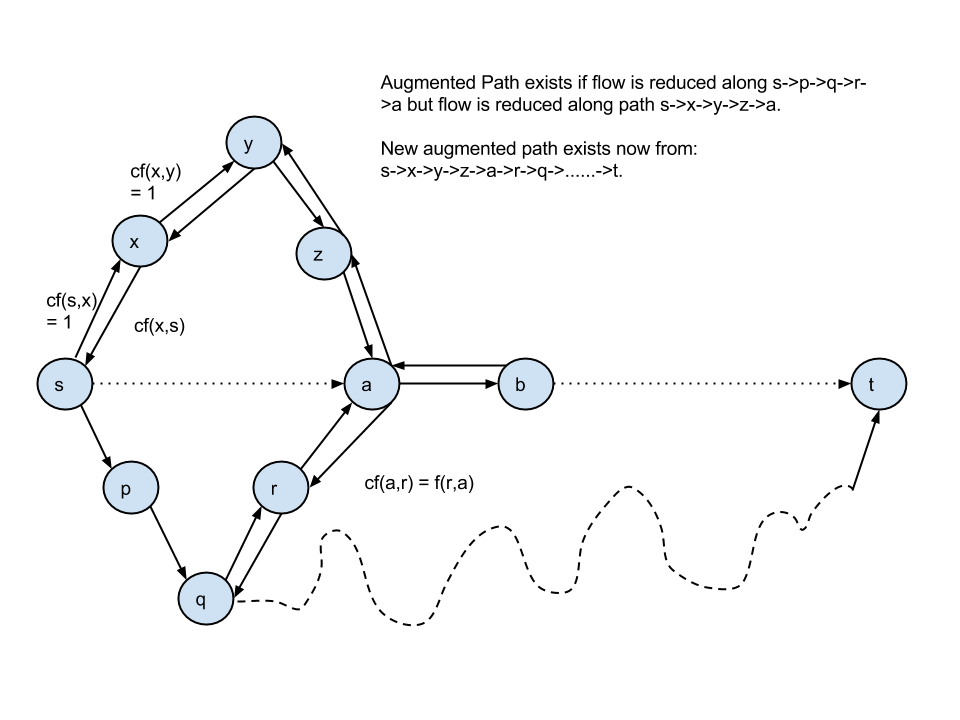
\includegraphics[scale=0.40]{1a}
    \caption{Proof of claim 1}
    \label{fig:1a}
\end{figure}
 
	As we have decreased flow across the first path, we have residual capacity of 1 available along all the edges of that path. Now as we have, a flow from r to a, $cf(a,r) = f(r,a) > 0$, $cf(r,q) = f(q,r) > 0$. So, we have an augmented path available from $s->x->y->z->a->r->q->.......->t$. This is different than the orginal path $s->p->q->......->t$, but still it is an augmented path with bottleneck of 1 and \textbf{it passes through a}. 
	
	
	Claim 2: After reducing the flow across one of the b to t path by 1, if there exists an augmented path from s to t, it will pass through b. 
	Proof: Exact same argument used in claim 1 can be used to prove claim 2. 
	
	Corollary: From the claim 1,2  and proof, we can infer that decreasing flow of 1 across any path from s to a and decreasing flow of 1 across any path from b to t,  will find the augmented path if one exists. Algorithm is based on this. 
	
	
	
			 		
	\begin{algorithm}[H]
	\caption{Update flow if capacity of one edge (a,b) is decreased by 1.}
	\label{alg:alg_decr_by_1}
	\begin{algorithmic}
	  	\If{$f(a,b) < C(a,b)$}
			\State $ f* $ $ is $ $ unchanged$ 	
		\EndIf
		\If{$f(a,b) == C(a,b)$}\\
			\State $C'(a,b) = C(a,b) - 1$
			\State $cf'(b,a) = 1$	
			\State $cf'(a,b) = -1$	
			\State Find out any path from s to a that carries some flow. ($flow >=1$). O(E)\\
			\State Reduce the flow across this path from s to a and update residual capacity.\\ 
			\State for all edges along selected s to a path O(E)
				\State $cf'(x,y) = cf(x,y) + 1$		\\
			\State Find out any flow path from b to t that carries some flow. ($flow >= 1$). O(E)\\
			\State Reduce the flow across this path from b to t and update residual capacity. \\
			\State for all edges along the selected b to t path O(E) 
				\State $cf'(x,y) = cf(x,y) + 1 $ \\
			\State Find out if an augmented path exists across the new residual  residual network. O(E)\\
			\If $there $ $exists $ $an $ $augmented $ $path $
			\State $f*$ is unchanged
			\Else
			\State $f* = f* - 1$
			\EndIf	
		\EndIf
	  	
	  	
	\end{algorithmic}
	\end{algorithm}

		
	\textbf{Running Time: O(3E) = O(E)		}
	
	
					
	
	

